

%----------------------------------------------------------------------------------------
%	CHAPTER 4: Socio-economic
%----------------------------------------------------------------------------------------

\chapter{FLR impacts on socioeconomic dimensions} \label{ch:socio}

The success or failure of a FLR project depends on both ecological and socioeconomic factors \cite{Le2012a, Meli2017b}. Forests and trees contribute in multiple ways through a variety of ecosystem services to alleviate poverty, reduce food insecurity and support sustainable livelihoods \citep{FaoNationalSurv}. Despite considerable proliferation of restoration actions across the globe, there is still little information on the links between FLR and socioeconomic conditions at local and regional levels \citep{Chazdon2008, Le2012a, Blignaut2013, Adams2016a, Lazos-Chavero2016}. As a consequence, the role of FLR for the national development remains underestimated and in some sectors invisible, preventing an optimal consideration in policy-making for social-ecological welfare. 

The most commonly used indicators of the impacts of FLR on socioeconomic dimensions are local income, local employment opportunities, other livelihood opportunities, food provision, stability of market prices, local empowerment and capacity building \citep{Le2012a}. Other approaches also include ‘avo-ided negative impacts’ (e.g. flood prevention or preservation of timber resources) as an indicator of socio-economic benefits. 

Especially in the last decade, a number of studies have analyzed and compared human dependence on tropical forests and environmental resources, mainly reporting case studies using various methodologies. The number of studies in Brazil is still meager and did not answer with certain to what extend and in which level FLR can impact socioeconomic benefits \citep{Adams2016a}. Therefore we performed a systematic review consolidating the existing literature regarding restoration, socioeconomic benefits and ecosystem services provision, and propose two strategies to include socio-economic aspects into spatial restoration prioritization in the Brazilian Amazon and Atlantic Forest biomes.

%%_________________________________________________________________
\section[\Large Literature Review  on socioeconomic dimensions]{Literature Review on FLR impacts on socio-economic dimensions} \label{sec:socio-lit}

Aiming to understand how FLR can impact socioeconomic aspects we conducted a systematic literature review on studies in Brazil, performed in two steps. First we used a set of broad word strings in Portuguese and English using Boolean searches (Restoration* AND Socio* OR Ecosystem services AND Brazil) for published articles in four databases (Scopus, Web of Science, Science Direct, Scielo and Periodicos Capes). That search resulted in 2.015 articles of which only 54 remained after a title and abstract assessment. To increase the number of articles we then used a set of specific word strings in Portuguese and English using Boolean searches (Food security OR Resilience OR Equity OR Health OR Poverty OR Empowerment OR Cultural OR Ecotourism AND Restoration AND Brazil) for published articles in the Web of science database. This second search retrieved 16 articles, all selected for the analysis. In total, both steps rendered 70 articles that were included in our literature database using the Mendeley software.

The majority of the restoration articles were case studies (86\%) mainly concentrated in the Atlantic forest (66\%) and the Amazon (20\%). The \ref{subsec:bio-revisão} subsection also found similar results indicating that ecological restoration in Brazil is essentially being based on the forestry biomes. 59\% of them used active restoration and 17\%\ focused on AgroForest Systems (AFS), techniques that fully need labour work and involvement of people and have direct impact on several socio-economic aspects. Most of the articles (64\%) identify restoration as having a positive impact on income (57\%), employment (32\%) and livelihood (31\%). The low percentage of well-being factors mentioned in the articles might be associated with the traditional restoration approaches that normally focused on financial and economic benefits, not including the human wellfare \cite{Dudley2005ForestContext}. No article specifically target the impacts of restoration on health, and very little mentioned cultural aspects and food security. The review also indicated, directly or indirectly, that restoration actions have a positive relation with several ecosystem services such as: biodiversity (41\%), water (27\%), soil formation (24\%), and climate regulation (23\%) (some studies indicated more than one) (Table \ref{table:socio}).
\newpage

\begin{table}
\caption{Different impacts of restoration on socioeconomic aspects in the Atlantic Forest and Amazon.}
% \begin{tabular}{lrrr} 
% \hline \hline 
% Intervention impact by 2030     	&Avoided deforestation   &Production loss &Additional profit \\
% (w.r.t. baseline projections)       &(million ha)   &(thousand ton.)     & \\ \hline 
% Cattle-ranching intensification (INT) &0      &0      &0\%    \\ 
% Timber processing units (FTY) &-0.9      &0      &47.9\%    \\ 
% Forest-Code compliance (FCC) &25.7      &-1.4      &-2.8\%    \\ 
% Combined interventions (SEM) &25.7      &-0.8      &46\%    \\ 
% \hline 
% \end{tabular}  


% \begin{document}
% \begin{table}[!h]
%   \centering % \begin{center}
%   \begin{tabular}{|c|c|c|c|} 
%   %\begin{tabular}{|p{2cm}|p{2.1cm}|p{3.5cm}|p{3.3cm}|p{1.6cm}|p{1.7cm}|p{1.7cm}|}
%     \hline
%     \bfseries Id Page  & \bfseries Politique de Partage & \bfseries Nombre Amis & \bfseries Nombre Pages qui ont reçu la pub \\
%     \hline
%     78 & Amis Seulement     & 23 &  23 \\
%     81 & Amis Seulement     & 25 &  25 \\
%     65 & Amis Seulement     & 25 &  25 \\
%     59 & Amis et leurs Amis & 26 &  51 \\
%     16 & Tout le Monde      & 27 & 100\\
%     45 & Amis et leurs Amis & 27 &  71 \\
%     69 & Amis Seulement     & 27 &  27 \\
%     74 & Amis Seulement     & 27 &  27 \\
%     99 & Amis Seulement     & 27 &  27 \\
%     30 & Amis et leurs Amis & 27 &  64 \\
%     \hline
%     \multicolumn{3}{|c|}{Moyenne des pages qui ont re\c{c}u  } & \\ % <---- inserted &
%     \hline  
%   \end{tabular}
%   %\end{center}


%\begin{tabular}{|l|l|} \hline
%    \pbox{20cm}{This is the first \\ cell} & second \\ \hline
%    3rd & and the last cell \\ \hline
%\end{tabular}

% \usepackage{array}
% \begin{document}
% \begin{tabular}{| c | c | >{\centering}m{5cm} |}
% Abc & Bcd & A long cell with text that wraps around and is centered
% \end{tabular}
% \end{document}

\scalebox{0.95}{
\begin{center}
\begin{tabular}{|m{5cm}|m{5cm}| >{\centering\arraybackslash} m{5cm} |} 
\hline
\multicolumn{2}{|c|}{\bfseries Socioeconomic outcomes variables} & \bfseries Cases with positive outcomes    \\ 
\hline
Income                          &   &40     \\ 
\cline{1-3}
Local employment opportunity    &   &23      \\ 
\cline{1-3}
Ecosystem provision services    &Food, Water, Biodiversity    &46         \\ 
\cline{1-3}
\cline{1-3}
(no-cash income)                &   &                 \\
\cline{1-3}
Productivity                    &Impact on pollination  &20  \\
\cline{1-3}
Well-being                      & Food security/Sovereignty, Resilience, Equity, Health, Poverty reduction, Empowerment       & 11 \\
\cline{1-3}
Livelihood opportunities  resources  &Agricultural intensification, Diversification, Migration Capital (natural, economic, financial, social, human)  & 22 \\
\cline{1-3}
Cultural                    &Cultural heritage, Spiritual and religious, Recreation and  ecotourism, Aesthetic and educational, Sense of place   &20   \\ \hline 
\end{tabular}
\end{center}
}


 \label{table:socio}
\end{table}


%________________________________________________________________

\subsection{\large FLR and well-being dimensions} \label{subsec:socio-well}

FLR seeks to restore not only large contiguous areas of degraded forest land, but also forest areas in rural landscapes, considering the multifunctionality of forests and its benefits for people. In Brazil, landowners need to restore their environmental debts as a legal obligation (Native Vegetation Protection Law/2012). However, restoration is a costly action as it means decreasing agricultural area (opportunity cost) and actively restoring - from fencing to planting seedlings (restoration cost). At the same time, food demand is increasing, so the challenge is to overcome the conservation versus production dichotomy, expanding forest cover while increasing food production in a sustainable manner and enhancing human well-being.

Clearly we depend on the land for food, shelter and a myriad of other ecosystem services (ES), but the quality of that land can affect our well-being in several ways (Bonn Challenge). Research in Brazil is mainly focus on biological process, with some initial work about the links between biodiversity and cultural and provision ecosystem services \citep{Pires2018}. While the importance of ES for human well-being is progressively well established and understood \citep{Leviston2018}, the interconnections between several aspects of well-being and their relation to FLR are still under-researched as we can see in Table \ref{sec:socio-lit}. There is  a lack of agreement and thus limited understanding about how to investigate, evaluate and incorporate well-being aspects into restoration approaches.
 
One important aspects of well-being is food security, and land and soil degradation pose significant challenges for food production, so it is essential to address cropland restoration in FLR approaches \citep{Pinto2014a}. FLR can have a positive impact on crops' productivity through the increase abundance of pollinators, for example (see Box \ref{Box4}). Also, biodiverse sucessional Agroforestry Systems (AFS) can produce a wide range of products, from fast growing horticultural crops (i.e. lettuce) to late sucessional trees. Tubenchlak \cite{Tubenchlak2017} collected data about species composition of 18 AFS in Rio de Janeiro state (Atlantic Forest biome), and found a great variation in the AFS, from 29 to 195 species including crops and native tree species. Also, in the northwest region of the state, transition to AFS allowed an increase and diversification of production, guaranteeing harvests throughout all months of the year, which was not feasible in the previous production system. These results highlight the importance of AFS to maintain not only biodiversity but also agrobiodiversity, and food security \cite{Tubenchlak2017}.


%The Millennium Ecosystem Assessment work (MEA 2005) divided the ES into four categories: provision, regulation, support and cultural, with closer links with well-being. Human well-being are influenced by many factors, such as health, security (food, water, energy) and basic material for a good life,  


%Access to green, natural areas, whether natural or restored, is found to improve child cognitive development and adult mental health 

%%%%%%%%%%%%%%%%%%%%%%%%%%%%%%%%%%%%%%%%%%%
% BOX Pollination
\addtocounter{mybox}{-1}

\begin{mybox}{Pollination increase food production in restored area}\label{Box4}
The analysis made in the TEEB Project (Box 3 in \ref{sec:water-qual} section) showed a high variation of pollinators abundance and visitation potential across landscapes, with higher abundance values for natural vegetation areas. The restoration scenarios (LC and SS) had higher mean abundances due to increased forest cover, which reflected in higher visitation potential values when compared to BAU. Comparing both restoration scenarios, maximum visitation potential values were higher in SS, as AgroForest Systems (AFS) had the highest abundance and visitation potential among land use classes. However, mean visitation potential values were higher in LC scenario, as scattered restoration increases landscape heterogeneity, decreasing flight distances between nesting habitat and floral resources. To assess the impact of these changes on agricultural productivity, we analyzed pollination dependency of 104 crops grown in the region: 40\%\ have some level of pollination dependency, 29\%\ have no dependency and 31\%\ have no data in literature. This means that between 40-70\%\ of the food crops might be affected by changes in pollinators occurrence and abundance, which highlights the importance of pollinators to a diverse and stable food supply.  When assessing the impact of the changes in visitation potential for 15 crops, productivity increased in LC and SS compared to BAU, with the biggest increment in AFS areas. The net value of pollination for 2035 was 15 million (R\$) in LC and 31 million in SS, indicating greater economic gain due to increment of production areas and pollination service. The scenarios show where and how decision makers could allocate restoration and sustainable strategies to support agriculture, contributing to biodiversity conservation and, food security, while and also boosting the economy in the Basin.
\end{mybox}

%________________________________________________________________
\subsection{\large FLR and cultural aspects} \label{subsec:socio-cult}

"Natural resources constitute the material foundation of cultural systems" \citep{Wehi2017}. In that sense, FLR should be implemented to satisfy not only conservation purposes but also socioeconomic values, including cultural ones. Cultural aspects are a part of the ecosystem services that are relevant constituents of human security, health and good social relations \citep{Arico2001}. It encompasses non-material values such as: spiritual, religious and aesthetic values, social relations, sense of place, recreation, tourism and cultural heritage \citep{Arico2001,Daniel2012}. 

Without considering these aspects, especially relationships between landscape and its stakeholders, restoration projects may not gain the social support needed for its success and may fail to deliver important benefits to ecosystems and to society. In the cultural facet, one must go deep into personal, heritage, religious and educational values through the perceptions and expectations of stakeholders \citep{Brancalion2014CulturalForest}. Those perceptions are important to understand local population' sense of place, and through it, elaborate public policies and social strategies to raise awareness, diminish the conflicts between local communities and governments and better implement restoration actions \citep{Ribeiro2009, Costa2013}.

Listening to and understanding local stakeholders' perception of the environment can be of great help to design FLR projects (see more in Box 5). For example, rural residents tends to use the forest for fruit collection since childhood, and this is a strong cultural link. Thus, the inclusion of edible trees in the project or even a AFS can boost the success of projects in such areas, making the  restoration more attractive and contributing to the acceptance of the population \citep{Muler}. FLR projects can also serve as recreation area for the local population. Lemgruber \cite{Lemgruber2017Luisa2017} found that residents saw the restored area as a place for leisure, and Carvalho (2016) register an increase of ecotourism in restored areas. Those actions help to value resident's historical context and local identity, maintaining the restored area and reducing possible conflicts \citep{Moom-SchultS.IFreitasSRPassarelli2014,Miranda2017}.

Despite its importance, cultural aspects remain poorly contemplated in restoration studies in Brazil (see Table \ref{table:socio}) and other parts of the world. A global meta-analysis that investigated the perception of stakeholders in restoration projects also found a lack of emphasis on cultural services, with only 3\%\ of the 1,589 studies mentioning cultural services \citep{Aronson2010}. 


Thus there is a crucial need to expand research relating cultural and restoration actions to better understand local stakeholders perception and use of the environment, their values and needs, increasing environmental awareness and mobilizing them in restoration and conservation of ecosystems \citep{Menzel2010, Lamarque2011, IIS2017EstudoPaulista}.

\newpage
%%%%%%%%%%%%%%%%%%%%%%%%%%%%%%%%%%%%%%%%%
%%%%% BOX teeb 1.4

\begin{mybox}{Including stakeholders perception in FLR projects}\label{Box5}
In the TEEB project (Box 3) maintaining cultural services (such as scenic beauty, beautiful flowers, contemplation, fruit supply, medicinal trees, bird attraction) were among the main drivers for local landowners to restore their properties. The forest was also positively and mainly associated with water benefits. However, several landowners based their cultural heritage as a barrier to change their activity to a more sustainable one or to restore areas, as forestry areas are still considered to be a waste of space in detriment of pastures and agriculture. On one hand, associating FLR with water production and quality might be the way to persuade landowner to restore, and on the other initiative to raise awareness and disseminate information is needed to overcome the cultural barriers. This survey  revealed the dichotomy of perceptions linked to cultural aspects among the local stakeholders, that can pave the way to better design FLR projects in the area.
\end{mybox}

%________________________________________________________________

\section{\Large Including social dimensions in spatial restoration planning } \label{sec:socio-spatial}

 The literature review emphasize the already growing notion among restoration professionals about the importance of including socioeconomic aspects in restoration planning. Restoration initiatives often neglect the needs of society for human and economic development and for food production, failing to be implemented \citep{DiMinin2017}. Restoration actions should be more directly associated to land-use planning in order to promote stakeholders' engagement and enhance the implementation of restoration actions (Pierce et al.2005). Furthermore, FLR projects can have a substantial impact on  households income, especially in poor areas \citep{Adams2016a, Jindal2012}, which is a huge concern in Brazil despite of poverty reduction in the last decades. 
 
 The Brazilian Gini index decreased from 0.637 to 0.575 between 1991 and 2010, a reduction of 9.7\%. A similar reduction was felt in the region embraced by the Atlantic Forest (9.6\%), but a subtler reduction (5.5\%) was felt in the Amazon. These biomes, therefore, could benefit from a FLR planning that accounts for social-economic benefits. 
 
 Also, restoration is a costly action as it means decreasing agricultural area (opportunity cost) and actively restoring - from fencing to planting seedlings (restoration cost). Therefore, developing restoration-models that includes economic yield might be a key step to implement restoration on the ground, meeting restoration and biodiversity targets.
 %  The earnings can come in form of employment, establishment of new activities (e.g. nurseries), government payments, selling forest products, agroforestry and cash crops products, and climate mitigation services, for example (Adams et al. 2016).
 For those reasons we are developing two approaches to include socio-economic aspects in our spatial prioritization maps, briefly described bellow.
 
 
\subsection{\large Income and Employment} \label{subsec:socio-income}

Income and employment are two outcomes most cited when evaluating the main aspects of socioeconomic impacts of FLR in the world \citep{Adams2016a} and in Brazil, according to section \ref{sec:socio-lit}. According to Calmon \cite{Calmon2011a} estimates, for every 1,000 hectares recovered, 200 direct and indirect jobs are created. In that sense, the 15 million hectares to be restored in the Atlantic Forest by law (NVPL) has the potential to generate more than 3 million direct and indirect local jobs through seed collection and processing, seedling production, planting and maintenance, not to mention ongoing monitoring and evaluation, and basic and applied research. 

Trying to assist in ebbing income inequality we aim to analyze and spatialize the benefits of FLR through job creation and its impacts on increasing income for vulnerable people in rural areas. So we are creating a socio-economical layer to be incorporated in a priorization model for restoration in the Atlantic Forest and Amazon. This layer will show the number of people who will come out of vulnerability or poverty condition due to the income and employment provided by restoration actions. The income data came from the IBGE's Demography Census \cite{20182018Contas2018} at district level, and we used the number of people in rural areas with less than half minimum wage, with no income statement and with ages between 18 and 59 years (economically active population).  


\subsection{\large Economical use of Legal Reserve} \label{subsec:socio-use}

Another more complex approach is to consider the use of economic species in the restoration of the Legal Reserve (LR). This strategy creates alternative sources of income for landowners while promoting the restoration and the compliance with environmental laws. We propose two models of LR restoration (Figures \ref{fig:modelmadeira} and \ref{fig:modelNTFP}) using species of commercial value based on planting schemes developed by the Laboratory of Tropical Forestry of the Luiz de Queiroz Higher School of Agriculture (LASTROP-ESALQ). The planting scheme uses $3x3$ spacing, totaling $1,111$ trees planted per hectare and a fallow cycle of timber species lasting 40 years.

We sought to incorporate spatial heterogeneity in species composition, productivity and price, with the aim of predicting, in a spatially explicit way, the potential economic return by planting native species of commercial value in LR. For that we did: i) an extensive literature review on species naturally occurring on the Amazon and Atlantic Rain Forest – including life cycle duration, Average Annual Increase, Productivity, Economic Value; ii) generate niche distribution models that indicate the potential area of occurrence of each species from a range of environmental predictors (eg, soil, climate, altitude); iii) estimate their density per individuals per hectare; and iv) calculate the potential gross economic value of all products produced during a 40 year cycle, including timber and non-timber forest products (NTFP).

In total, we found the necessary information on 143 species, 66 occurring in the Amazon, 105 in the Atlantic Forest, and 30 occurred in both biomes. 102 species are used exclusively for timber, 21 are used only for NTFP extraction and 19 are used for both. Furthermore, 46 of those species are used for food, which can have positive impacts on food security and sovereignty. 

 
 \begin{figure}
\centering
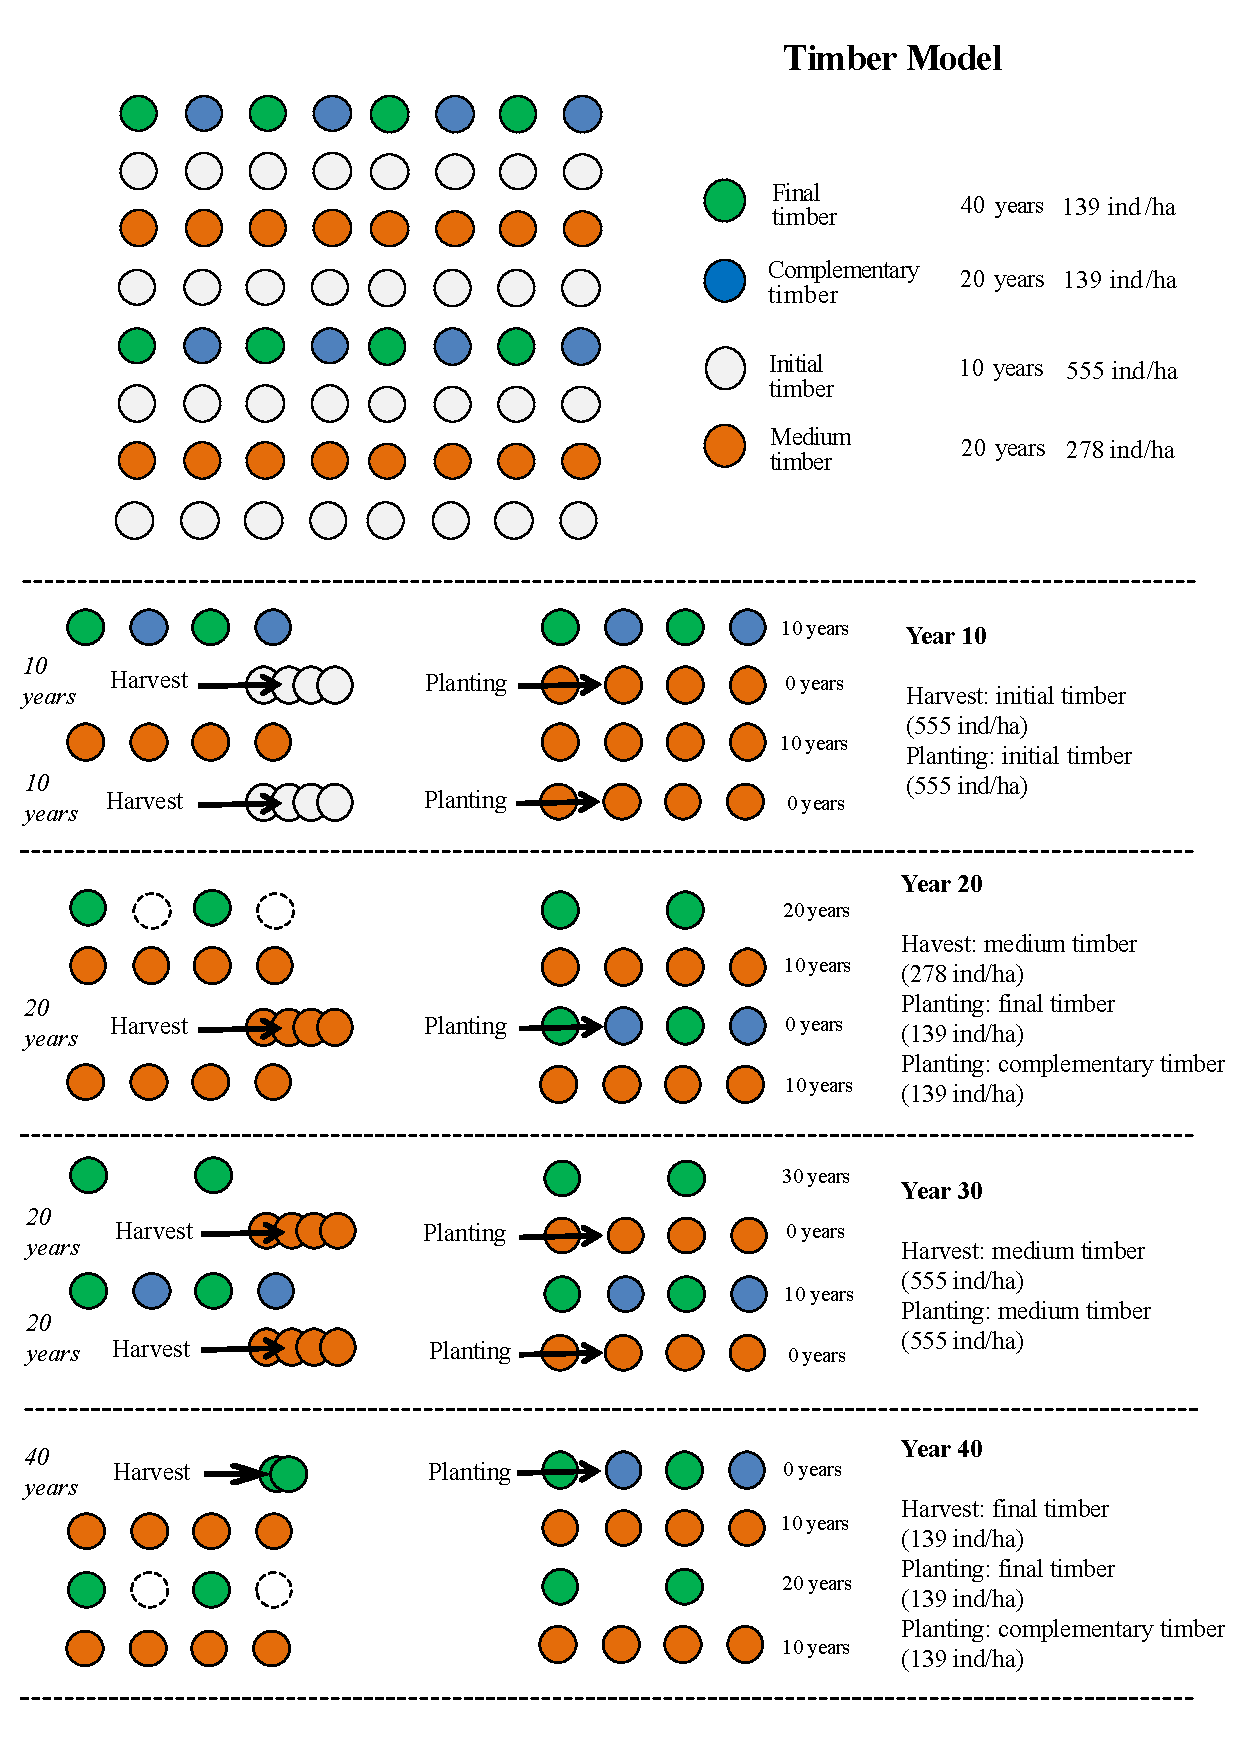
\includegraphics[width=\textwidth]{pictureve/socio-modelomadeira.pdf}
\caption{Economic exploitation model of Legal Reserve exclusively with timber species. }
\label{fig:modelmadeira}
\end{figure}

  \begin{figure}
\centering
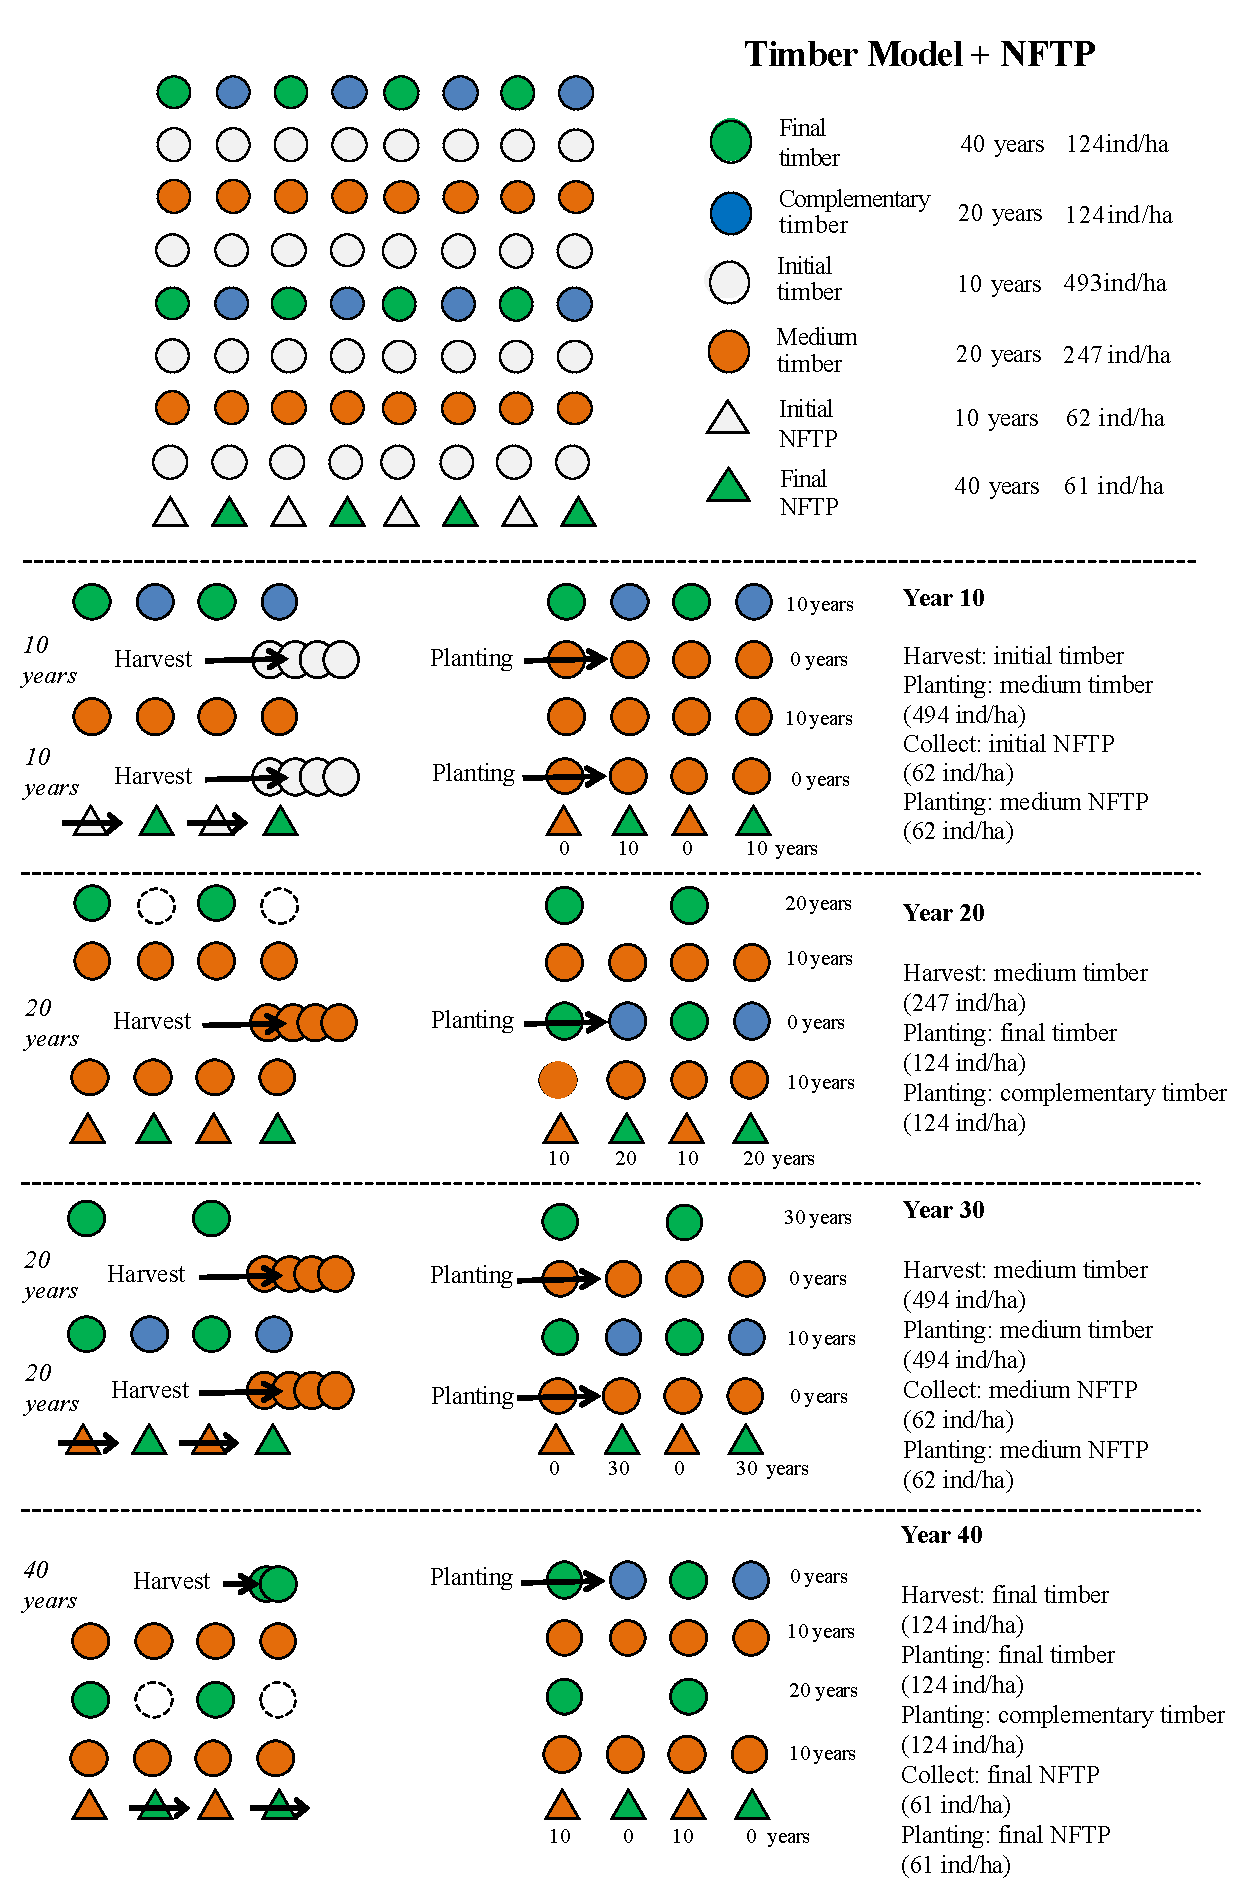
\includegraphics[width=\textwidth]{pictureve/socio-modeloNTFP.pdf}
\caption{Economic exploitation model of Legal Reserve with timber species and non timber forest products (NTFP).} \label{fig:modelNTFP}
\end{figure}